% discuss numerical simulation - transfer from L1 to the Moon type orbit
% compare with the transfer using invariant manifolds
\section*{}
\subsection*{Numerical Simulation}
\begin{frame} %-----------------------------------------------%
\frametitle{Transfer example}
\begin{itemize}
	\item Transfer from \( L_1 \) to region near Moon
	\item Generate reachable set using computational geometric optimal control over fixed horizon
	\item Invariant manifold transfer serves as baseline
\end{itemize}
	\begin{figure} 
	\centering 
	\begin{subfigure}[htbp]{0.5\textwidth} 
		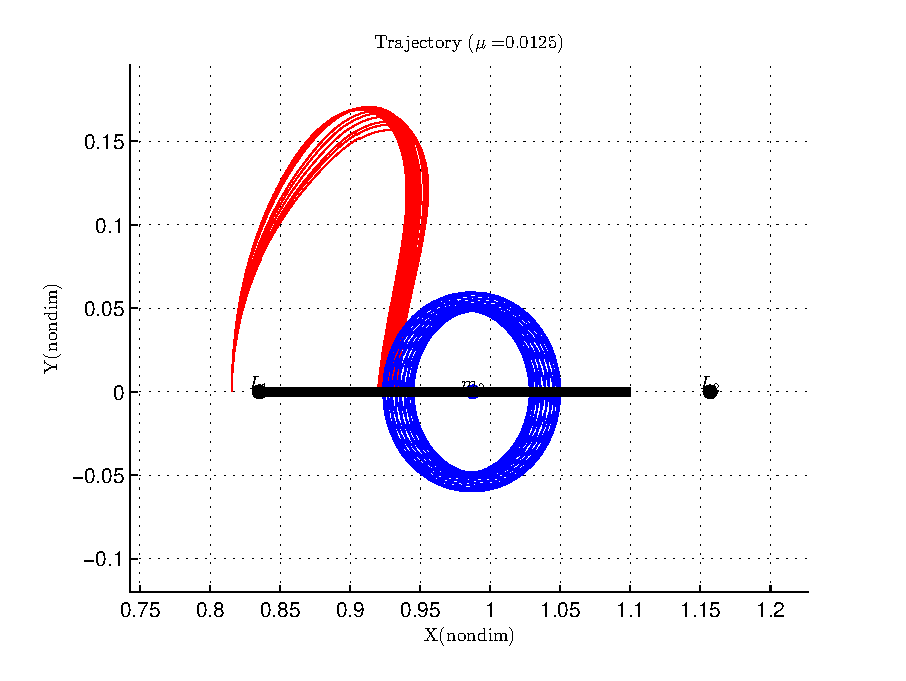
\includegraphics[width=\textwidth]{reach_trajectory}  
	\end{subfigure}~
	\begin{subfigure}[htbp]{0.5\textwidth} 
		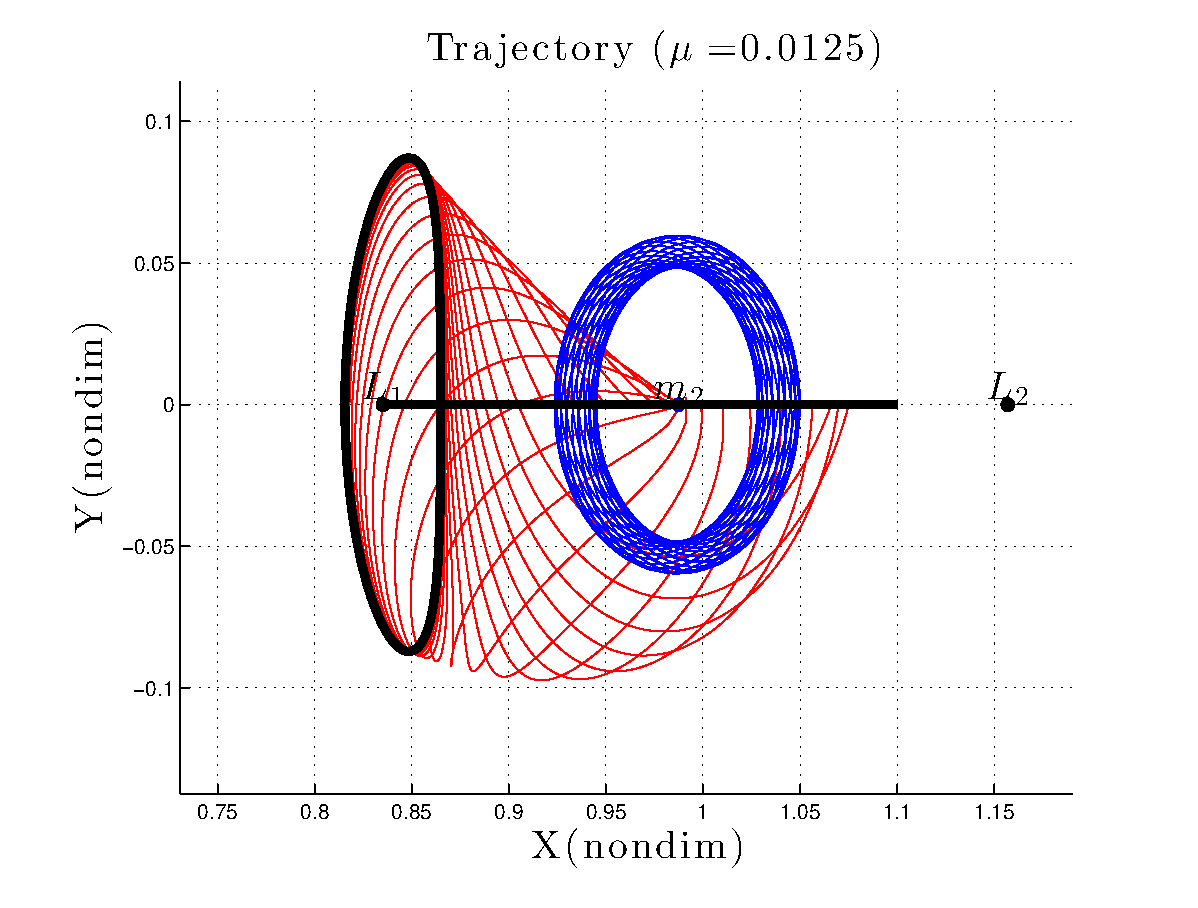
\includegraphics[width=\textwidth]{manifold_trajectory} 
	\end{subfigure} 
	\end{figure}
\end{frame} %------------------------------------------------%

\begin{frame}%------------------------------------------------%
\frametitle{Transfer Example}
\begin{itemize}
	\item Reachable set is generated on Poincar\`e section
	\item Invariant manifold does not always allow for transfer
	\item Low-thrust propulsion allows for intersection
	\item Intersection state ( \( \bar{x}_t \)) and Jacobi integral used to determine optimal transfer
\end{itemize}
\begin{figure}
	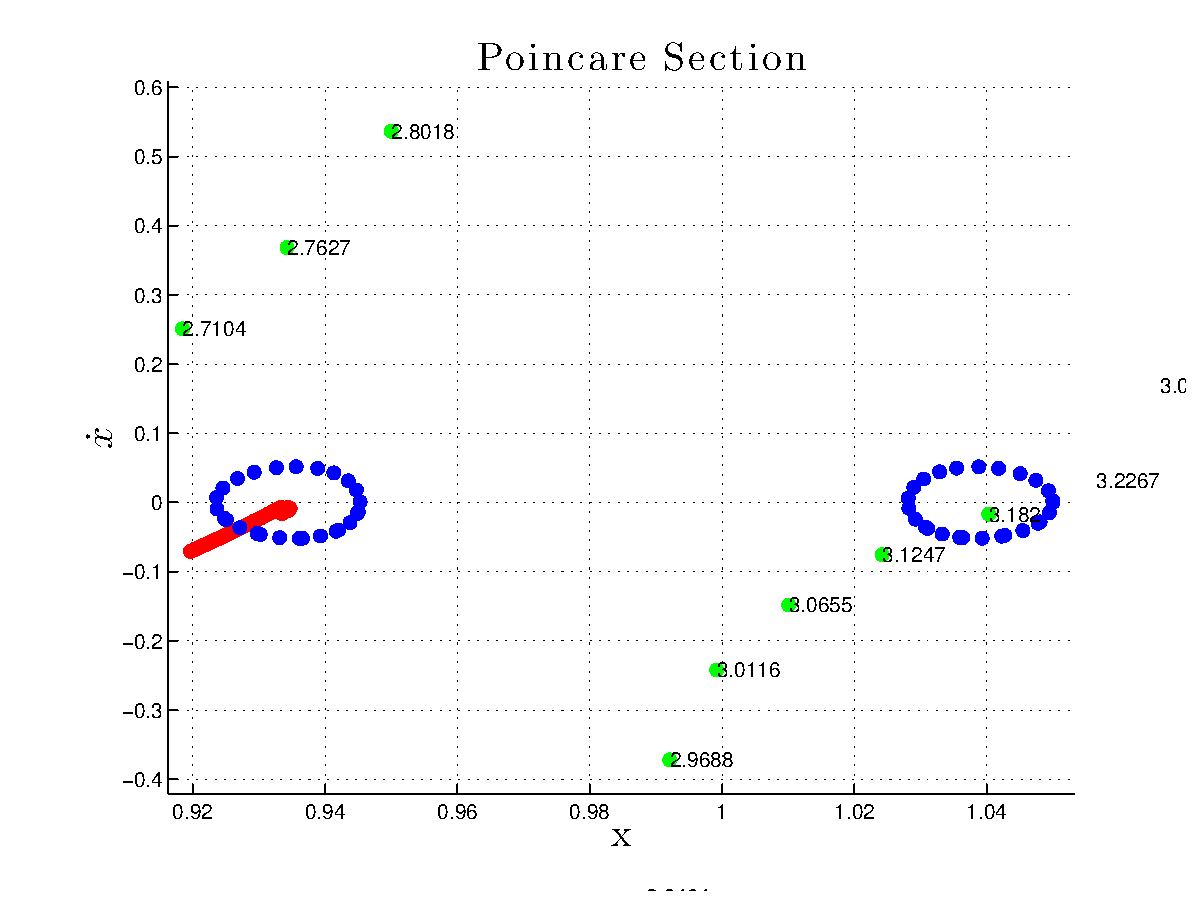
\includegraphics[width=0.5\textwidth]{poincare_compare}
\end{figure}
	Reachable set TOF = 1.4
	Invaraint Manifold TOF = 3.1
\end{frame} %--------------------------------------------------%